\section{Circuits at sub-domain granularity}

\begin{figure}[h]
  \centering
  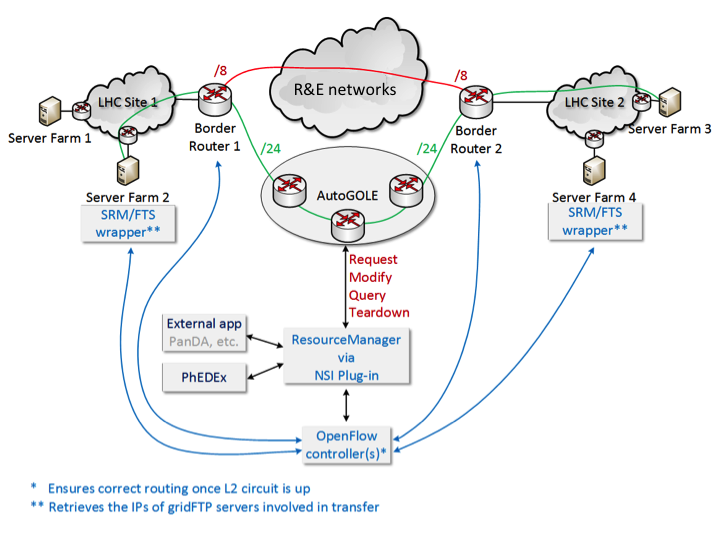
\includegraphics[width=0.95\textwidth]{figure-proposed-solution-global}
  \caption{The middleware view of the proposed solution. The ResourceManager requests NSI circuits and informs OpenFlow controllers of their existence. The SRM/FTS wrapper at each site informs the OpenFlow controller of the transfers that are actually taking place. The OpenFlow controller dynamically updates the sites' routing to steer the appropriate traffic into the circuit.}
  \label{fig:proposed-solution-global}
\end{figure}

\begin{figure}[h]
  \centering
  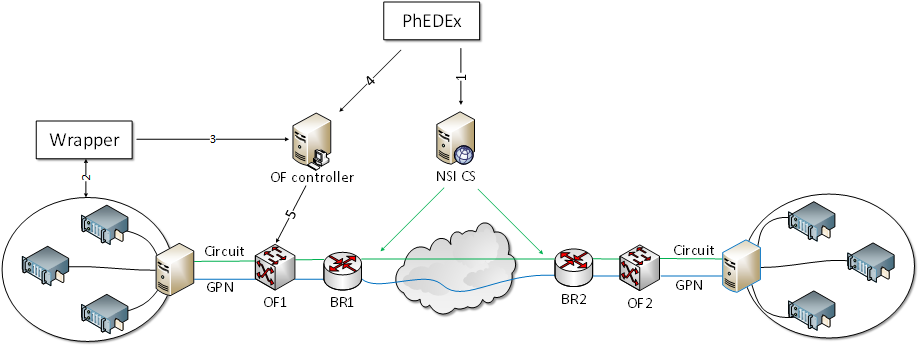
\includegraphics[width=0.95\textwidth]{figure-proposed-solution-detail}
  \caption{Workflow of the proposed solution. PhEDEx requests a circuit, meanwhile the wrapper script is constantly informing the OpenFlow controller of the files that are in transfer at any moment. Once PhEDEx has a circuit, it informs the OpenFlow controller of its existence, and the controller diverts the relevant traffic to use the circuit.}
  \label{fig:proposed-solution-detail}
\end{figure}

As mentioned, not all the traffic between two sites should necessarily go via a circuit, should one exist. Typically, sites have a cluster of data-servers which host data, and any or all of them may participate in a given bulk transfer between two sites.

To build circuits at granularity finer than the IP domain of the participating sites, it is important to know the exact set of data-servers that will serve or receive the data. PhEDEx itself may not have access to that information. PhEDEx constructs the SURL for the source and destination from its own knowledge, but the SURL typically points to a gateway-host that redirects the transfer to the actual hosts that will take part, exactly analogous to a web-site redirecting a URL. PhEDEx does not see this `Transfer URL', or TURL, because it invokes the transfer tool (FTS, FDT etc) with the SURL, and it is this transfer tool that is redirected to the appropriate TURL.

Our proposed solution is illustrated in figures~\ref{fig:proposed-solution-global} and \ref{fig:proposed-solution-detail}. In figure~\ref{fig:proposed-solution-global}, the experiment-specific middleware is either PhEDEx or the `External app', which communicates with the ResourceManager to request circuits. The ResourceManager is independent of the experiments, and can become part of the WLCG middleware. This component already exists, having been refactored from the original prototype reported in \ref{ANSE_ISGC_2014}. The ResourceManager communicates with OpenFlow network controllers, telling them of the creation or destruction of NSI circuits and the list of files that are to be transfered over the circuit.

A wrapper-script runs on the data-servers at the sites, wrapping the calls to gridFTP so it can intercept them without having to modify gridFTP itself. The wrapper notifies the same OpenFlow network controllers that a transfer is about to start. The OpenFlow controllers then modify the routing table at the sites to divert the traffic onto a circuit, if one exists.

While non-trivial, this solution does not require privileged software to run on the sites data-servers, and cleanly separates the experiments from the network management layer. The use of a wrapper script to talk to the OpenFlow controllers means that the underlying transfer technology (gridFTP or whatever) does not have to be modified. It does require that OpenFlow controllers be installed at participating sites, but once there, they offer a single point of control for the circuit behaviour, making the system easier to understand and debug.

Figure~\ref{fig:proposed-solution-detail} shows more detail of the workflow involved. PhEDEx (or some other experiment middleware) requests an NSI circuit, which is established between the sites border routers. Meanwhile, the wrapper script is constantly informing the OpenFlow controller of the set of files being transfered at any point in time. This is all the OpenFlow controller needs to know when to establish a level-3 circuit from the data-server to the border router and over the level-2 circuit to the destination.




















Given that PhEDEx itself is essentially a steering component, using underlying transfer tools such as FTS and FDT to manage the actual transfers, 